\documentclass{article}
\usepackage[utf8]{inputenc}
\usepackage[spanish]{babel}
\usepackage{listings}
\usepackage{graphicx}
\graphicspath{ {images/} }
\usepackage{cite}

\begin{document}

\begin{titlepage}
    \begin{center}
        \vspace*{1cm}
            
        \Huge
        \textbf{Taller Memoria}
            
        \vspace{0.5cm}
        \LARGE
        Taller - Nociones de la memoria del computador
            
        \vspace{1.5cm}
            
        \textbf{Johan David Rojas Martinez}
            
        \vfill
            
        \vspace{0.8cm}
       
        \Large
\begin{figure}[h]

\includegraphics[width=4cm]{logoudea.png}
\centering
\end{figure}

        \vfill
        Despartamento de Ingeniería Electrónica y Telecomunicaciones\\
        Universidad de Antioquia\\
        Medellín\\
        Septiembre de 2020
                 
    \end{center}
\end{titlepage}

\tableofcontents

\section{Introduccion}
Mediante este documento se estara realizando respuesta a algunas preguntas acerca del funcionamiento de la memoria,veremos cual es en general la definicion de memoria de un computador, mencionaré los tipos de memoria que conozco y lo que conocia de estas antes de investigar, se mostraran algunas imagenes para ilustrarnos mejor de lo que estamos hablando,tambien estaremos abordando como es la manera en que se gestiona una memoria y que hace que unas memorias sean mas rapidas que otras. 

\section{Preguntas} \label{contenido}

\subsection{Defina que es la memoria del computador.}
la memora del computador es un dispositivo muy importante para llevar a cabo el correcto funcionamiento de este y segun lo entendido sin esta el ordenador ni siquiera podria arrancar, la memoria tiene la capacidad de retener, almacenar y memorizar datos, en este dispositivo se almacena temporalmente la informacion que mas tarde sera utilizada por el microprocesador, esa informacion realiza un proceso muy particular en nuestra computadora, ya que primero es almacenda en un dispositivo que tiene una alta capacidad de almacenamiento, pero que es mas lento que otros dispositvos(Disco duro), luego se toma una porcion de esta informacion y es ubicada temporalmente en la memoria RAM(como se habia dicho anteriormente) donde se ubica para poder trabajar, se toma una porcion de los documentos ubicados en la memoria para que el microporocesador haga su trabajo, como ejecutar una serie de instrucciones, calculos necesarios o alguna orden que se le envie, posteriormente esa informacion que ya ha sido manipulada se envia a otro lugar de la memoria donde se ubican los documentos ya procesados, este proceso se repite varias veces con todos los documentos que se encuentran apilados en en la memoria a una velocidad muy rapida que el humano nunca percibiria, finalemnte cuando ya no hay mas nada que procesar esos docuementos se regresan al disco duro. 

\vspace{0.5cm}
Este dispositivo se interconectada a la unidad central de procesamiento (CPU, por las siglas en inglés de Central Processing Unit) y los dispositivos de entrada/salida, implementan lo fundamental del modelo de computadora de la \textbf{arquitectura de Von Neumann.}\cite{geniolandia}

\vspace{0.5cm}
la memoria se divide en gran numero de piezas pequeñas llamadas células. Cada ubicacion o celda tiene una direccion unica que varia desde cero hasta el tamaño de la memoria menos uno. por ejemplo, si el ordenador tiene 64 k palabras, entonces esta unidad de momoria tiene 64*1024=65536 posiciones de momoria. La direccion de estos lugares varia de 0 a 65535. \cite{tutorialspoint}


\subsection{Mencione los tipos de memoria que conoce y haga una pequeña descripción de cada tipo.}
Los tipos de memoria que conozco y los que he escuchado desde que empecé a utilizar computadores son: Memoria RAM, disco duro y memoria caché.
\subsubsection{Memoria RAM}
Antes de haber investigado y leer el informe que habia sido enviado por el profesor mi idea acerca de la memoria RAM es que era un dispositivo que iba colocado en la placa madre(mother board) del computador y se encargaba de permitirnos abrir varios programas o pestañas en nuestro computador, teniendo tambien la idea de que entre mas memoria RAM tuviera nuestro ordenador iba a ser muchisimo mas rapido, pues mi idea era que la memoria RAM era la encargada de la velocidad de nuestro PC.

\vspace{0.5cm}
Tras haber investigado y leido el informe ya me hago una idea mas clara de lo que es la memoria RAM y basicamente es como un escritorio donde ubicamos una informacion temporalamente que despues sera utilizada por el microprocesador y se ubica en un espacio de memoria con una direccion exclusiva, entonces tal vez mi idea de que a mas memoria RAM mas veloz era el computador no era del todo erronea, ya que si por ejemplo contamos con un escritorio bastante amplio(Memoria RAM), se pueden realizar las tareas con mas comodiad y podemos alamecenar mucha mas informacion sin enredos y con suficiente espacio(es una analogia que puede servir para entender como funciona). La memoria RAM almacena la informacion en binarios(1 y 0) suele ser mas rapida que otros dispositivos de memoria porque se puede acceder a su informacion de una forma mas rapida y no tan compleja esto se debe a que la informacion es guardada forma aleatoria, un dato que me parecio bastante curioso fue que la memoria RAM es un semiconductor rápido de almacenamiento de datos con tiempos de acceso que oscilan entre 5 a 12 nanosegundos. Contiene todos los procesos del sistema de funcionamiento de una computadora. \cite{geniolandia}

\subsubsection{Disco duro}
Lo que entendía por disco duro es que este es un dispositivo electronico y que parte de su funcionamiento es de forma mecanica, se encuentra ubicado dentro de la torre del ordenador, donde se almacena y se guarda la informacion de la computadora, nuestros archivos se encuentran ahi de forma permanentemente ahi aunque apaguemos nuestro PC, estos los podemos encontrar en el mercado con distintas capacidades de almacenamiento, por ejemplo: 250GB, 500GB, 1TB,etc,entre mas capapacidad tenga nuestro disco duro mas informacion y archivos podemos tener en nuestra computadora y es en este mismo donde tenemos instalado nuestro sistema operativo que es el que nos permite poder interactuar con la maquina y los dispositivos perifericos de una manera amigable y entendible. El disco duro suele ser uno de los dispositivos mas lento que tiene nuestro computador pero a su vez uno de los mas amplios en memoria. 

\vspace{0.2cm}

El principal funcionamiento de un disco duro se basa en que los cabezales pongan marcas magnéticas en las pistas del plato con 3 posiciones diferentes estas pueden ser: 1, 0 ó neutro y las maquinas son capaces de decodificar ese código binario como información. Al momento de guardar un archivo en el disco duro de nuestro PC, este escribe en los platos una secuencia de unos y ceros a velocidades que se miden en micro segundos. \cite{qloudea}
\vspace{0.2cm}

\emph{Acontinuacion se muestra una imagen de como es fisicamente un disco duro}(\ref{fig:disco_duro})

\begin{figure}[h]
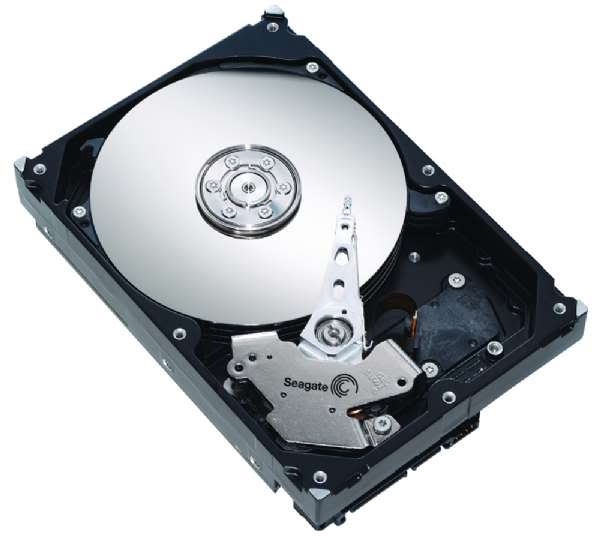
\includegraphics[width=6cm]{disco_duro.jpg}
\centering
\caption{Imagen del disco duro}
\label{fig:disco_duro}
\end{figure}

\subsubsection{Memoria caché}
La memoria caché segun lo que entendí de la definicion del documento que nos envio el profesor Augusto \cite{Augusto} es que esta se utiliza para trabajar con la informacion que el microprocesador nota que es utilizada de forma muy seguida, entonces para este no tener que buscarla de nuevo y ejecutar siempre esas mismas instrucciones la guarda en la memoria caché y puede reutilizarla cuantas veces quiera, esta memoria es mucho mas rapida que las mencionadas anteriormente,pero a su vez tiene un alto costo y cuentan con poca capacidad de almacenamiento(12 megabytes).

\vspace{0.3cm}

Los computadores modernos han venido incorporando esta nueva tecnologia en tres niveles(L1 ,L2,L3), la memoria L1 se encuentra incorporada dentro de los nucleos del microprocesador y es una de las mas rapidas pero con menos capacidad de almacenamiento esta se divide en dos partes una para datos y otra para instrucciones cada una de estas cuenta con 32 kilobytes, la memoria caché L2 hoy en dia los fabricantes tambien la incorporan dentro de los nucleos del microprocesador en comparacion con la L1 es un poco mas lenta,pero con mas almacenamiento, ya que cuenta con 256 kilobytes de capacidad para almacenar datos e instrucciones, finalmente la memoria caché L3 se encuentra incorporada dentro del procesador pero fuera de los nucleos y es la mas lenta de todas (sin dejar de ser mas rapida que la memoria RAM que se encuentra instalada en la \textbf{motherboard}),esta es la que cuenta con mas capacidad de las 3 memorias caché contando con una capacidad de 12 MB. 

\subsection{Describa la manera como se gestiona la memoria en un computador.}

\subsection{¿Qué hace que una memoria sea más rápida que otra? ¿Por qué esto es importante?}

\section{Conclusión} \label{conclulsion}

\bibliographystyle{IEEEtran}
\bibliography{references}

\end{document}
